\def\mytitle{MATRICES USING PYTHON}
\def\myauthor{T.VARSHA REDDY}
\def\contact{varshareddy724@gmail.com}
\def\mymodule{Future Wireless Communication (FWC)}
\documentclass[10pt, a4paper]{article}
\usepackage[a4paper,outer=1.5cm,inner=1.5cm,top=1.75cm,bottom=1.5cm]{geometry}
\twocolumn
\usepackage{graphicx}
\graphicspath{{./images/}}
\usepackage[colorlinks,linkcolor={black},citecolor={blue!80!black},urlcolor={blue!80!black}]{hyperref}
\usepackage[parfill]{parskip}
\usepackage{lmodern}
\usepackage{tikz}
	\usepackage{physics}
%\documentclass[tikz, border=2mm]{standalone}
%\usepackage{karnaugh-map}
%\documentclass{article}
\usepackage{tabularx}
%\usepackage{circuitikz}
\usepackage{enumitem}
\usetikzlibrary{calc}
\usepackage{amsmath}
\usepackage{amssymb}
\renewcommand*\familydefault{\sfdefault}
\usepackage{watermark}
\usepackage{lipsum}
\usepackage{xcolor}
\usepackage{listings}
\usepackage{float}
\usepackage{titlesec}
\providecommand{\mtx}[1]{\mathbf{#1}}
\titlespacing{\subsection}{1pt}{\parskip}{3pt}
\titlespacing{\subsubsection}{0pt}{\parskip}{-\parskip}
\titlespacing{\paragraph}{0pt}{\parskip}{\parskip}
\newcommand{\figuremacro}[5]{
   % \begin{figure}[#1]
    %    \centering
     %   \includegraphics[width=#5\columnwidth]{#2}
      %  \caption[#3]{\textbf{#3}#4}
     %   \label{fig:#2}
    %\end{figure}
}

\newcommand{\myvec}[1]{\ensuremath{\begin{pmatrix}#1\end{pmatrix}}}
\let\vec\mathbf
\lstset{
frame=single, 
breaklines=true,
columns=fullflexible
}
%\thiswatermark{\centering \put(181,-119.0){
\includegraphics[scale=0.13]{iith_logo3}} }
\title{\mytitle}
\author{\myauthor\hspace{1em}\\\contact\\FWC22038\hspace{6.5em}IITH\hspace{0.5em}\mymodule\hspace{6em}Assignment}
\begin{document}
\maketitle
\tableofcontents
\section{Problem}
\textbf{A circle touches the line y=x at a point P such that OP=4$\sqrt{2}$, where O is the origin. The circle contains the point (-10,2) in its interior and the length of its chord on the line x+y=0 is 6$\sqrt{2}$}
 
\section{Figure}
  %\includegraphics[scale=0.47]{matrix.pdf}
  \includegraphics[scale=0.5]{/home/srinath/Documents/matrix.pdf} 
  	\begin{center}
  Figure of construction
  	\end{center}
\section{Solution}

Let c($\alpha$,$\beta$) be the center of the circle touching OP at P and making intercept AB = 6$\sqrt{2}$  on the line x+y=0.\\
If r is the radius of the circle then\\
\\
In $\Delta$ACL
\begin{center}
$r^2 = \vec{\norm{A-C}^2} = \vec{\norm{C-L}^2 + \norm{L-A}^2}$....(1) 
\end{center}
\begin{align*}
\vec{\norm{C-L}^2} = \vec{\frac{n^TP-C}{\norm{n}}}\\
\end{align*}
%Given
\begin{center}
$ \vec{\norm{L-A}}$=3$\sqrt{2}$\\
 \end{center}
n =$ \begin{pmatrix}1\\1\\ \end{pmatrix}$, 
$n^T$ =$ \begin{pmatrix}1 \hspace{0.2cm}1 \end{pmatrix}$, 
P =$ \begin{pmatrix}\alpha\\ \beta\\ \end{pmatrix}$, 
$\vec{\norm{n}} = \sqrt{2}$,c = 0\\
Given\\
$\vec{\norm{A-L}^2} = \vec{\norm{3\sqrt{2}}}$\\
substitute  all above equation in (1) \\
\\
In $\Delta$OCP\\r=5$\sqrt{2}$
\begin{center}
$\vec{\norm{O-C}^2} = \vec{\norm{C-P}^2 + \norm{P-O}^2}$....(2) \\
\end{center}
Given\\
$\vec{\norm{O-C}^2} = \vec{{\alpha}^2 + {\beta}^2}$,\\
$\vec{\norm{C-p}^2} = r^2$,\\
$\vec{\norm{P-O}}$ = 4$\sqrt{2}$\\
Solve equation (1) ,(2)\\
\begin{center}
$\alpha$ - $\beta$ = +/- 10....(3)\\
\end{center}
Distance from center to x-y=0 line\\
\begin{align*}
\vec{\norm{C-P}^2} = \vec{\frac{n^TP-C}{\norm{n}}}\\
r^2 = \frac{(\alpha-\beta)^2}{2}....(4)\\
\end{align*}
$n^T$ = $\vec{\begin{pmatrix}1 \hspace{0.2cm}-1 \end{pmatrix}}$, 
P =$\vec{ \begin{pmatrix}\alpha\\ \beta\\ \end{pmatrix}}$, 
$\vec{\norm{n}} = \sqrt{2}$,c = 0\\
Solve equation (3),(4)\\
\begin{center}
then r=5$\sqrt{2}$....(5)\\
Substitute equation (5) in (1)\\
we get\\
$\alpha$ = -9 , $\beta$ = 1\\
$\alpha$ =  9 , $\beta$ = -1\\
$\alpha$ =  1 , $\beta$ = -9\\
$\alpha$ = -1 , $\beta$ = 9\\
The standard equation of the conics is given as :
we choose $\alpha$ and $\beta$ values from which the line passes through the point (-10,2)\\
so, $\alpha$= -9 and $\beta$=1
 
\begin{align}
\vec{x}^{\top}\vec{V}\vec{x}+2\vec{u}^{\top}\vec{x}+f=0
\end{align}
Where
$\vec{Vx}$ = 
$\begin{pmatrix}
1 & 0\\
0 & 1
\end{pmatrix}$,
$\vec{u}$=$\vec{ \begin{pmatrix}-9 \\1 \end{pmatrix}}$, 
f = 32.
\end{center}
\section{Construction}
We considered midpoint as L on the chord AB, from that we found the distance between the center to L.And also given OP length,Again from centre to OP finding the distance. 
\begin{align*}
\vec{\norm{C-P}^2} = \vec{\frac{n^TP-C}{\norm{n}}}\\
\end{align*}
\begin{align*}
\vec{\norm{C-L}^2} = \vec{\frac{n^TP-C}{\norm{n}}}\\
\end{align*}
from the above 2 equations we get the centre and radius of the circle.
$\alpha$ = -9 , $\beta$ = 1\\
r=5$\sqrt{2}$
\end{document}


